%%& -job-name=08-gov

%%%%%%%%%%%%%%%%%%%%%%%%%%%%%%%%%%%%%%%%%
% Beamer Presentation
% LaTeX Template
% Version 1.0 (10/11/12)
%
% This template has been downloaded from:
% http://www.LaTeXTemplates.com
%
% License:
% CC BY-NC-SA 3.0 (http://creativecommons.org/licenses/by-nc-sa/3.0/)
%
%%%%%%%%%%%%%%%%%%%%%%%%%%%%%%%%%%%%%%%%%

%----------------------------------------------------------------------------------------
%	PACKAGES AND THEMES
%----------------------------------------------------------------------------------------

\documentclass[xcolor=table, envcountsect,12pt]{beamer}
\setbeamertemplate{theorems}[numbered]
\mode<presentation> {
	
	% The Beamer class comes with a number of default slide themes
	% which change the colors and layouts of slides. Below this is a list
	% of all the themes, uncomment each in turn to see what they look like.
	
	%\usetheme{default}
	%\usetheme{AnnArbor}
	%\usetheme{Antibes}
	%\usetheme{Bergen}
	%\usetheme{Berkeley} %
	%\usetheme{Berlin} %
	%\usetheme{Boadilla}
	%\usetheme{CambridgeUS} %
	%\usetheme{Copenhagen}
	%\usetheme{Darmstadt}
	%\usetheme{Dresden} %
	%\usetheme{Frankfurt}
	%\usetheme{Goettingen}
	%\usetheme{Hannover}
	\usetheme{Ilmenau} %
	%\usetheme{JuanLesPins}
	%\usetheme{Luebeck}
	%\usetheme{Madrid}
	%\usetheme{Malmoe}
	%\usetheme{Marburg}
	%\usetheme{Montpellier}
	%\usetheme{PaloAlto} %
	%\usetheme{Pittsburgh}
	%\usetheme{Rochester}
	%\usetheme{Singapore}
	%\usetheme{Szeged}
	%\usetheme{Warsaw}
	
	% As well as themes, the Beamer class has a number of color themes
	% for any slide theme. Uncomment each of these in turn to see how it
	% changes the colors of your current slide theme.
	
	%\usecolortheme{albatross}
	%\usecolortheme{beaver}
	%\usecolortheme{beetle}
	%\usecolortheme{crane}
	%\usecolortheme{dolphin}
	%\usecolortheme{dove}
	%\usecolortheme{fly}
	%\usecolortheme{lily}
	%\usecolortheme{orchid}
	%\usecolortheme{rose}
	%\usecolortheme{seagull}
	%\usecolortheme{seahorse}
	%\usecolortheme{whale}
	%\usecolortheme{wolverine}
	
	%\setbeamertemplate{footline} % To remove the footer line in all slides uncomment this line
	%\setbeamertemplate{footline}[page number] % To replace the footer line in all slides with a simple slide count uncomment this line
	\setbeamertemplate{footline}[text line]{%
  		\parbox{\linewidth}{\vspace*{-8pt}NONCONFIDENTIAL - EXTERNAL\hfill\insertshortauthor\hfill\insertshorttitle}}
	\setbeamertemplate{navigation symbols}{} % To remove the navigation symbols from the bottom of all slides uncomment this line
}
\usepackage{etex}

%%--
\usepackage{graphicx} % Allows including images
\usepackage{booktabs} % Allows the use of \toprule, \midrule and \bottomrule in tables
%%--
\usepackage{url}
\usepackage{soul}
\usepackage{xcolor}
\usepackage{lipsum}
\usepackage[normalem]{ulem}
\usepackage{amsmath}
\usepackage{amsthm}
\usepackage{amssymb}
\usepackage{graphicx}
\usepackage{epstopdf}
\usepackage{multicol}
\usepackage{multirow}
\usepackage{color}
\usepackage{threeparttable}
\usepackage{caption}
\usepackage{subcaption}
\captionsetup{compatibility=false}
\DeclareMathOperator*{\argmax}{arg\,max}
\theoremstyle{remark}
\newtheorem*{rem}{Remark}
\theoremstyle{theorem}
\newtheorem{prop}{Proposition}
\usepackage{pdflscape}
\usepackage{afterpage}
\setcounter{MaxMatrixCols}{34}
\usepackage{dcolumn}
\usepackage{geometry}
\usepackage{tikz}
\usetikzlibrary{shapes.arrows, positioning}
%%-----------------------------------------------------------------------------------
\makeatletter
%%%%%%%%%%%%% Textclass specific LaTeX commands.
%\makeatletter
\theoremstyle{plain}
\newtheorem{lem}{Lemma}
\newtheorem{cor}{Corollary}
\newtheorem{conjecture}{Conjecture}
%%
\makeatletter
\beamer@theme@subsectionfalse
\makeatother
%
%CUSTOM COMMAND FOR BLUE URLs
\newcommand{\myul}[2][black]{\setulcolor{#1}\ul{#2}\setulcolor{black}}
%
%
%-----------------------------------------------------------------------------------------
%----------------------------------------------------------------------------------------
%	TITLE PAGE INFO
%----------------------------------------------------------------------------------------
\title{Liquidity Shocks in Virtual Markets}
\author{Caleb Bray}
\date{May 14, 2026}
\vspace{.2in}

%------------------------------------------------
\begin{document}
	% title page
	\begin{frame}
		\titlepage
		
		\centering \tiny All views and opinions shared here are my own and do not represent those of the KC Fed or Federal Reserve System.
	\end{frame}
%------------------------------------------------
%------------------------------------------------
%------------------------------------------------
	
	
%--------------------------------------------------------------------------------------------------
%	DEVELOPMENTS
%--------------------------------------------------------------------------------------------------
\section{Introduction}
	
\begin{frame}
	\frametitle{}
	\begin{itemize}
		\item 
		\item 
		\item 
	\end{itemize}

\end{frame}

\begin{frame}{Obtaining ``Skins''}
\begin{center}
\vspace{-2mm}
\begin{tikzpicture}[
    every node/.style={inner sep=0pt}
]
    % Top image
    \node (img1) {
        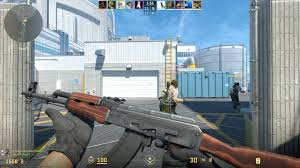
\includegraphics[scale=0.45]{default_ak.jpg}
    };
    
    % Bottom image (smaller gap)
    \node[below=2cm of img1] (img2) {
        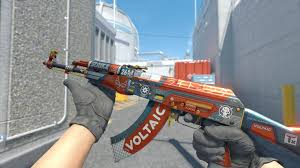
\includegraphics[scale=0.45]{bloodsport_ak.jpg}
    };
    
    % Middle point
    \path (img1.south) -- (img2.north) coordinate[midway] (middle);
    
    % Downward arrow with wider body
    \node[
        single arrow,
        draw=black,
        fill=black,
        minimum height=2cm,
        minimum width=0.3cm,
        single arrow head extend=0.1cm,
        single arrow tip angle=90,
        anchor=center,
        rotate=-90,
        inner sep=0.3cm
    ] (arrow) at ([yshift=0.15cm]middle) {};
    
    % Overlay image (shifted up 0.3cm)
    \node at (arrow.center) {
        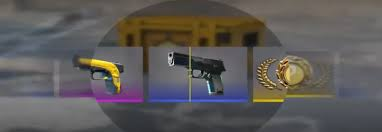
\includegraphics[scale=0.25]{case_opening.jpg}
    };
    
\end{tikzpicture}
\end{center}
\end{frame}

\end{document}
	
	%--------------------------------------------------------------------------------------------------
	%	THEMES
	%--------------------------------------------------------------------------------------------------
	\section{}
	
%	\begin{frame}
%		\frametitle{}	
%		\begin{figure}
%			\centering
%			\makebox[0pt]{\includegraphics[scale=0.6]{}}
%		\end{figure}
%	\end{frame}
	
%	\begin{frame}
%		\frametitle{.}	
%		\begin{figure}
%			\centering
%			\makebox[0pt]{\includegraphics[scale=0.57]{}}
%		\end{figure}
%	\end{frame}

%	\begin{frame}
%		\frametitle{}	
%		\begin{figure}
%			\centering
%			\makebox[0pt]{\includegraphics[scale=0.45]{}}
%		\end{figure}
%		\tiny 
%	\end{frame}

	%--------------------------------------------------------------------------------------------------
	%	REVISIONS
	%--------------------------------------------------------------------------------------------------

	%--------------------------------------------------------------------------------------------------
	%	APPENDIX
	%--------------------------------------------------------------------------------------------------
	\section{Appendix}
	
\end{document}
